\documentclass[10pt,twocolumn,letterpaper]{article}

\usepackage{cvpr}
\usepackage{times}
\usepackage{epsfig}
\usepackage{graphicx}
\usepackage{amsmath}
\usepackage{amssymb}
\usepackage{enumitem,epsfig,algorithm,algpseudocode}


\usepackage{listings}
\usepackage{color}

\definecolor{dkgreen}{rgb}{0,0.6,0}
\definecolor{gray}{rgb}{0.5,0.5,0.5}
\definecolor{mauve}{rgb}{0.58,0,0.82}

\lstset{frame=tb,
  language=Python,
  aboveskip=3mm,
  belowskip=3mm,
  showstringspaces=false,
  columns=flexible,
  basicstyle={\small\ttfamily},
  numbers=none,
  numberstyle=\tiny\color{gray},
  keywordstyle=\color{blue},
  commentstyle=\color{dkgreen},
  stringstyle=\color{mauve},
  breaklines=true,
  breakatwhitespace=true,
  tabsize=3
}

% Include other packages here, before hyperref.

% If you comment hyperref and then uncomment it, you should delete
% egpaper.aux before re-running latex.  (Or just hit 'q' on the first latex
% run, let it finish, and you should be clear).
\usepackage[breaklinks=true,bookmarks=false]{hyperref}

\cvprfinalcopy % *** Uncomment this line for the final submission

\def\cvprPaperID{****} % *** Enter the CVPR Paper ID here
\def\httilde{\mbox{\tt\raisebox{-.5ex}{\symbol{126}}}}

% Pages are numbered in submission mode, and unnumbered in camera-ready
%\ifcvprfinal\pagestyle{empty}\fi
\setcounter{page}{1}
\begin{document}

%%%%%%%%% TITLE
\title{Traffic Anomalies Detection with Object Tracking}
\author{
Daniel Shumaker\\
Michigan State University\\
{\tt\small shumak37@msu.edu}
% For a paper whose authors are all at the same institution,
% omit the following lines up until the closing ``}''.
% Additional authors and addresses can be added with ``\and'',
% just like the second author.
% To save space, use either the email address or home page, not both
\and
Luan Nguyen\\
Michigan State University\\
{\tt\small nguye590@msu.edu}
\and
Pengyu Chu\\
Michigan State University\\
{\tt\small chupengy@msu.edu}
}

\maketitle
%\thispagestyle{empty}

%%%%%%%% ABSTRACT
\begin{abstract}
   Anomaly detection is an important field in creating a smart city. This helps automatically detect unusual actions such as lane violation, illegal U-turns, driving against traffic, etc. In this paper, we proposed a fusion approach by combining both detection and tracking to solve the problem of anomaly detection. Specifically, we developed models for car detection, road detection, and vehicle tracking. Based on the relative position between cars, the road, and the cars' velocity, we were able to identify the occurrence of anomalies. Experimental results show that our approach achieves decent accuracy for Track 3 of the AI City Challenge competition.
\end{abstract}

\section{Introduction}
The opportunity for cities to use traffic cameras as citywide sensors to optimize traffic flow and manage disruptions is immense. Currently, we are lacking an ability to track vehicles over large areas that span multiple cameras at different intersections in all weather conditions. To achieve this goal, one has to address three distinct but closely related research problems: 1) Detection and tracking of targets within a single camera, known as multi-target single camera (MTSC) tracking; 2) Re-identification of targets across multiple cameras, known as ReID; and 3) Detection and tracking of targets across a network of cameras, known as multi-target multi-camera (MTMC) tracking. MTMC tracking can be regarded as the combination of MTSC tracking within cameras and image-based ReID with spatio-temporal information to connect target trajectories between cameras. Since the goal of the competition is to develop a new approach for better car detection and tracking as well as anomaly detection, we aim to propose a novel model for anomaly detection from highway video cameras.

\section{Problem Description}
Our project comes from \textit{aicitychallenge.org}: a competition held every year that challenges programmers to expand our society's knowledge in the realm of self driving cars with a focus on urban car automation. Every year they offer new challenges. Our project is based on challenge number $3$ - \'Traffic Anomaly Detection\'. Like the name suggests, our challenge is to detect behavior that deviates from the way vehicles normally act. Examples of anomalies that we are looking for are illegal lane crossing, wrong direction driving, swerving cars, illegal U-turns, stopped vehicles, and crashes with a few stretch goals like detecting the lack of headlight usage and excessive breaking. Since the ability to detect those activities depends heavily on the data set quality, the developed model must be robust to a wide range of situations such as zooming, vibrations, and sudden direction changes. Most of the videos in the challenge are retrieved from highway cameras. Thus, a place where U-turn detection will be hard to train due to the infrequency of their occurrence in the given data.

This problem is important because it can help save the lives of people as cars more and more become autonomous. With sensors tracking traffic, signaling systems, and infrastructure, our transportation systems are becoming smarter. With computer vision and deep learning, there are many opportunities to solve real-world problems with data gained from multi-cameras. The major causes of accidents are the outliers to normal drivers. The drivers that go much slower on the free way, that aggressively change lanes, and ride others' bumpers are a major cause for sober accidents. Another major accident is caused by drivers under the influence of drugs. These drivers have a differing, and more dangerous set of driving patterns. Both groups can be extremely dangerous, particularly in traffic highways and intersections. With software that can detect anomalies in behavior, a computer could spot potential hazards and, depending on where it is implemented, could notify police in the area of a potentially drunk driver, or could tell an autonomous vehicle which cars to give a wide berth to. Solutions could potentially get the humans in the loop to pay attention to meaningful visual information in situations where timely intervention can save lives \cite{naphade2017nvidia}.

Unfortunately, progress has so far been limited for several reasons like missing data labels, and the lack of high-quality models that convert data to decent forms. In other words, it is hard to get data with labels from the real world. Due to the lack of labels, anomalies cannot be classified with current algorithms. Thus, we plan to seek a semi-supervised approach to address this problem and focus on the research and development of techniques that rely more on transfer learning and semi-supervised learning. 

By using pre-trained models like VGG 16 \cite{ren2015faster}, we can leverage transfer learning to combine these models with our approach and detect the abnormal traffic behaviors from traffic camera video data which is provided by NVIDIA corporation.

\section{Related works}
There are not many previous works in anomaly detection regarding highway videos. Giannakeris \etal \cite{giannakeris2018speed} calculated speed of running cars to detect the differences in speed among different cars on the road to determine the unusual things. However, this way of calculating depends heavily on the accuracy of the car detection and tracking. If one of these terms are not correct, it can dramatically lead to wrong results. Zhang \etal \cite{zhang2019deep} used deep neural network to summarize video and process anomaly. This approach seems to be stable to noise and zoomed scenarios. However, it needs to process the whole video several times to summarize and analyze the results. To fuse the results of different camera viewpoints, Tang \etal \cite{tang2018single} utilized a tracking module to keep track of each car on the road. They further estimate speed based on 3D features of visual and semantic meaning. Wei \etal \cite{wei2018unsupervised} proposed an unsupervised approach that makes the model to be near real-time processing. The key idea of this approach is based on the background modeling which finds the differences between frames. All of the mentioned approaches are either easily sensitive to moving cameras or have insufficient capacity to process long video. Our approach uses a fusion of supervised and non-supervised learning to minimize those defects and obtain decent results.

\section{Data Set}
Our solution to the problem described above begins with the data set we have to work with. \textit{AI City Challenge} provided us with the data for this challenge. The training and test set are visually pretty similar. Each folder contains 100 mp4 files. Each video is about 15 minutes long, usually is set in a highway, and, not surprisingly, has a lot of cars in it. In the README file for the training videos, the challengers give us the areas they believe to have issues. Surprisingly, most videos in these sets don't have any anomalies in them, or at least were not recorded in the README document. 

From watching videos in the data set, we found that it is very likely that there will be wind, and the video will need to be stabilized before processing. The cameras used to record the videos differ in quality greatly. There are many factors that vary in different videos such as weather condition, the time of day the filming took place, geographical location, and the angle of the cameras. Another observation we made after looking at the videos, and at the suggested anomalies of the training videos, was a lack of diversity in the errors. Most of the errors that were recorded are related to stalled vehicles stopped on the sides of the road, and many of the errors that are not about stalled vehicles, do not appear to have any errors at all.

To get a good result and make models stable, we apply preprocessing techniques to normalize the data. Figure \ref{train17} shows a few images from the videos in the data set. An example of an image with an anomaly in it is presented in Figure \ref{train2}.

\begin{figure}  
    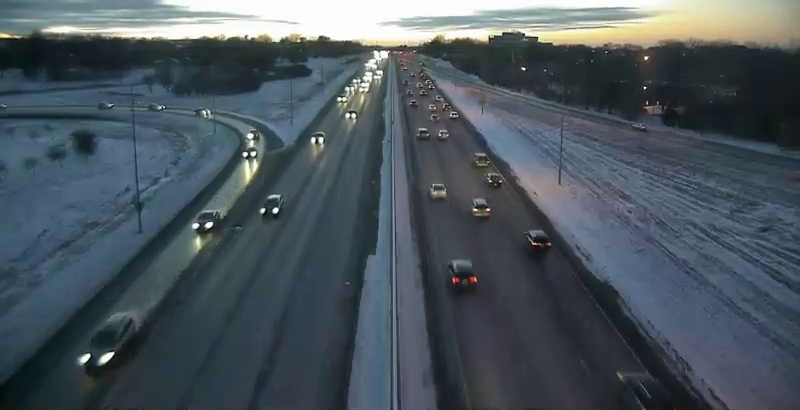
\includegraphics[scale=.29]{images/anomalyTrain17.png}
    \caption{Image from video 17}
    \label{train17}
\end{figure}

\begin{figure}  
    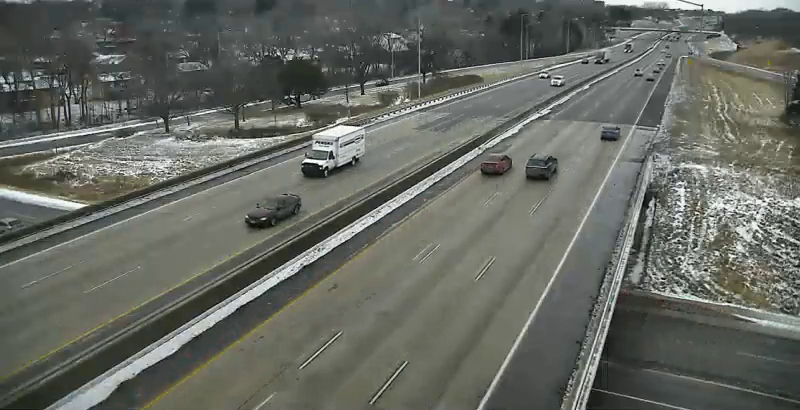
\includegraphics[scale=.29]{images/anomalyTrain41.png}
    \caption{Image from video 41}
    \label{train41}
\end{figure}

\begin{figure}  
    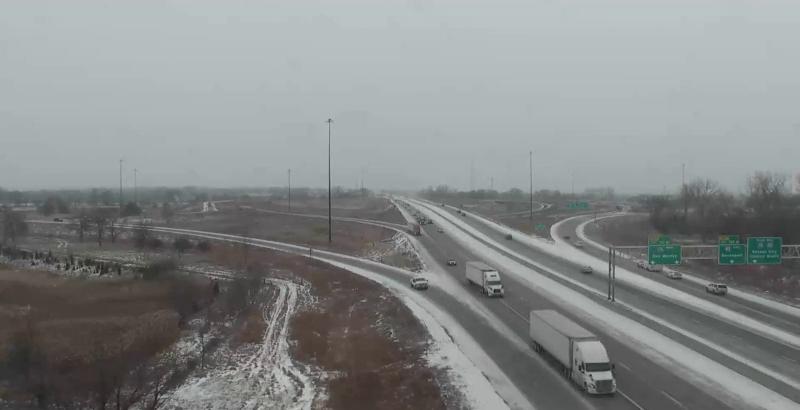
\includegraphics[scale=.29]{images/anomalyTrain66.png}
    \caption{Image from video 66}
    \label{train66}
\end{figure}

\begin{figure}  
    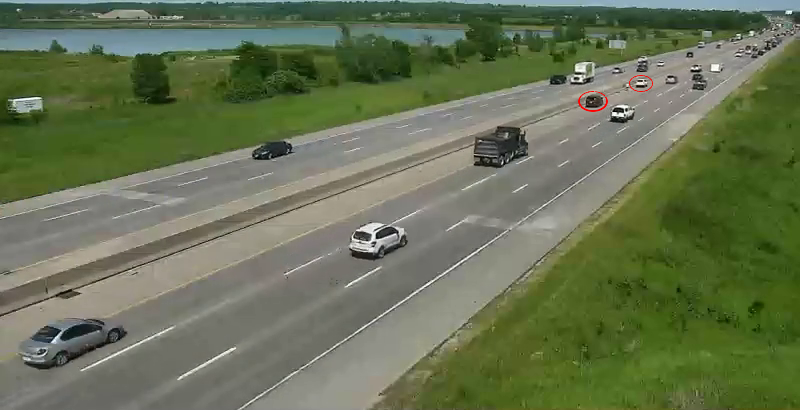
\includegraphics[scale=.29]{images/anomalyTrain2_focus.png}
    \caption{Image from video 2. Contains Anomalies. In the small red circles, two cars are stopped on the side of the road.}
    \label{train2}
\end{figure}


The challengers require that we report our anomalies in the same way that they do: give the video name, the start time of the anomaly, and the end time of it in seconds. If the anomaly continues past the end of the video, we are to give the last second of the video as the stopping time.


\section{Proposed method}

Based on the definition of anomalies, we mainly have two types of anomalies, which are running off the road and stalling on the highway. The following criteria are the guide that we used to develop our model:

\begin{itemize}
	\item Detect all cars or trucks in the videos and point out their locations; 
	\item Track these vehicles in the sequence of each video; 
	\item Measure the speed of cars based on a continues frames in the videos and judge its status; 
	\item Detect the road area to check whether a car runs off the road or not. 
\end{itemize}

In this section, we introduce our methods mentioned in details.

\subsection{Vehicle Detection}

In the realm of objective detection, we have lots of state-of-the-art methods including two-stage detection methods like Faster R-CNN \cite{ren2015faster} or one-stage detection represented by YOLOv3\cite{redmon2018yolov3}
and SSD\cite{liu2016ssd}. After a comparison among these methods, we chose Mask R-CNN as our detector because it had the best accuracy over the benchmark.\cite{DBLP:journals/corr/HeGDG17}.

To increase the stability of the model, we use two state-of-the-art stages: object detection and semantic segmentation CNN, and Mask R-CNN \cite{DBLP:journals/corr/HeGDG17} with ResNet101 as the backend. In addition, for improving the detection accuracy, we annotated 498 images extracted from these videos to train our own model to specifically detect cars.
	
\subsubsection{Train the Custom Model}

Mask R-CNN is a very popular instance segmentation architecture in the computer vision. It can rapidly improve object detection and semantic segmentation results over a short period of time. This method is conceptually intuitive and offers flexibility, robustness, and fast training and inference time if we start from a pre-trained model. This important structure is displayed in figure \ref{maskrcnn}. Our goal in this work is to utilize the comparably enabling framework for vehicles segmentation and get their bounding boxes.

	\begin{figure}  
    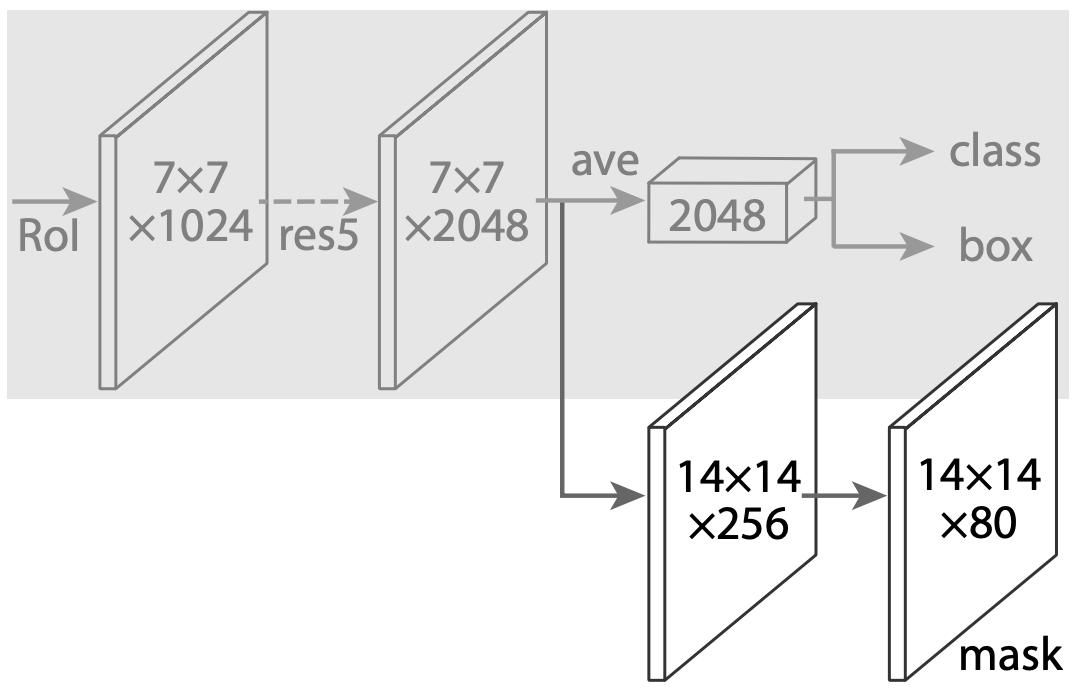
\includegraphics[width=8cm]{images/maskrcnn.png}
    \caption{The head architecture in Mask R-CNN Structure with ResNet}
    \label{maskrcnn}
	\end{figure}

Because it is hard to train a CNN model from scratch, we used the pre-trained model in the COCO data set\cite{DBLP:journals/corr/LinMBHPRDZ14}, which is a public images data set, to detect cars in our scene. However, after some attempts, we found the pre-trained model cannot fit our situation well in what may have lots of dense environment. In addition, we also have many overlapping conditions among cars and the object sizes shift a lot responding to the figure \ref{annotated_car}. 
	
	\begin{figure}  
    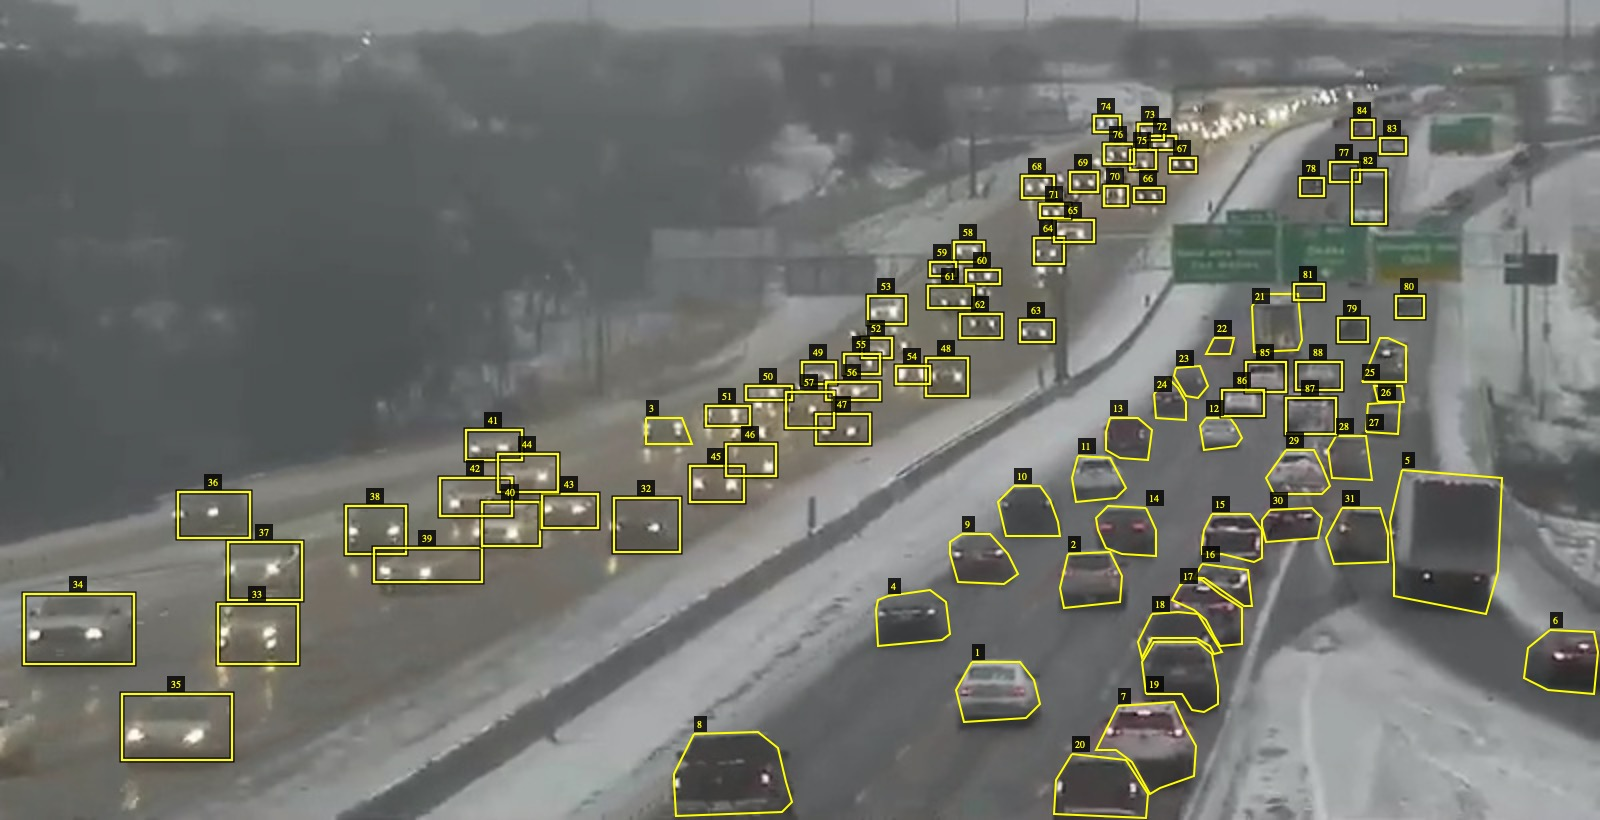
\includegraphics[width=8cm]{images/annotated_car.jpg}
    \caption{Vehicle annotation}
    \label{annotated_car}
	\end{figure}
	
In our algorithm for anomaly detection, vehicle detection is the most important part, so we extract 500 frames from the 100 videos over the training data set. For the balanced test, we eliminate some unclear ones and add some noise where there is no vehicle. Then we use SGD (Stochastic Gradient Descent) to train the parameters in the pre-trained model. Actually, we only updated the classification and mask layer. Both of which are the final layer of our CNN model, as well as the RPN part in the figure \ref{maskrcnn}. This speeds it up and after 60 epochs, we get a decent result with 0.917 accuracy that is over 0.84 accuracy in the pre-trained model. Currently, we ignore small vehicles that consist of only 3 or 4 pixels because it's still hard to annotate manually.


\subsubsection{Detect Vehicles with Mask R-CNN}

After getting our custom model of CNN, we can use it to label vehicles in the videos. Because Mask R-CNN is designed for images, we needed to extract frames from the videos and use those for detection. Fortunately, python has a video library named 'moviepy' to deal with this problem. With 'moviepy', we extract a sequence of frames from each video, detect vehicles one by one and then reconstruct them to a new video as our output, which means we apply the detector on each frame. To save time, we sped up the original videos to 10x. More details will be displayed in the code. Figure \ref{seq_cars} displays an example of a continuous result. 
	
	\begin{figure}  
    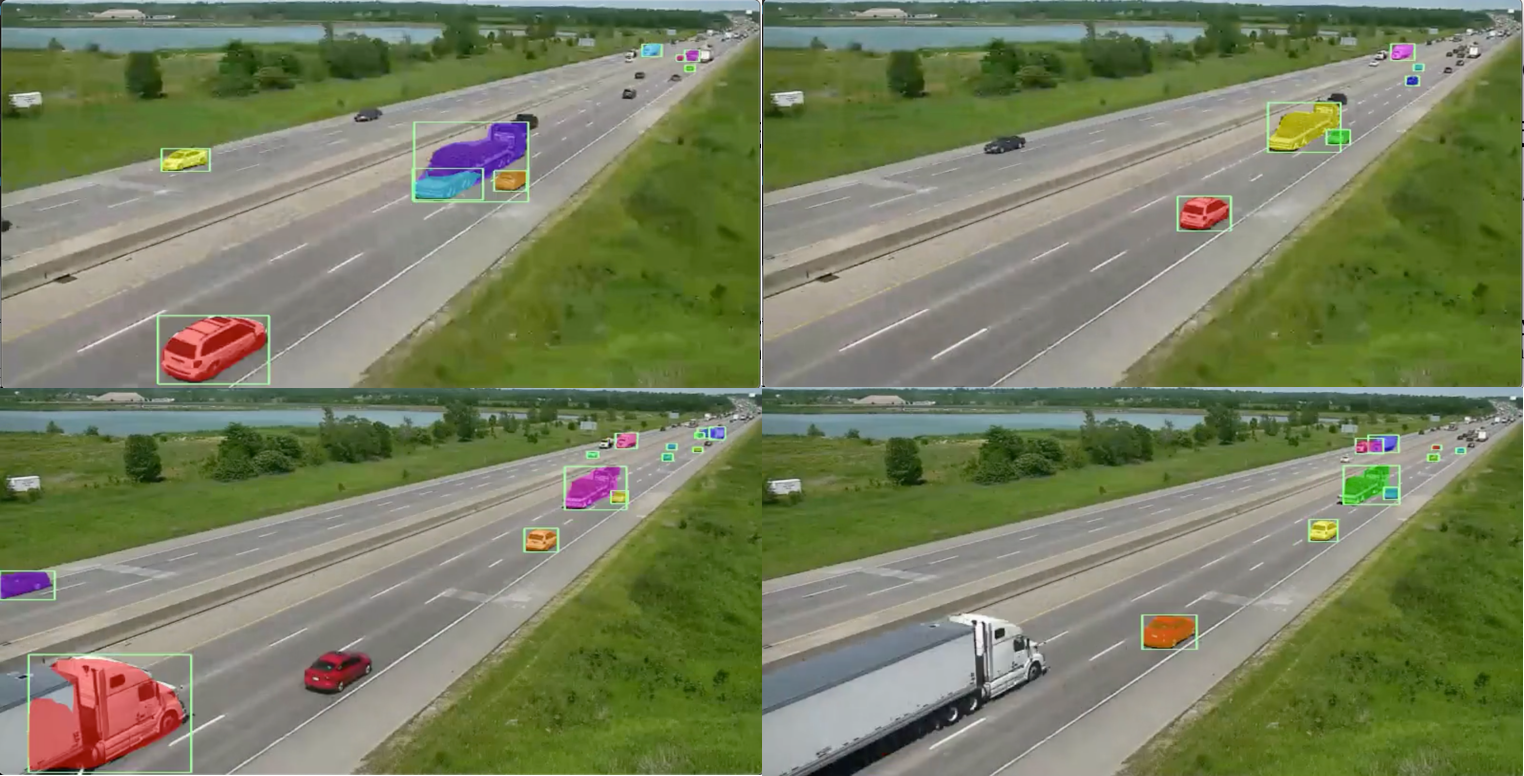
\includegraphics[width=8cm]{images/car.png}
    \caption{Detect cars through videos with Mask R-CNN. The sequence is from left to right and top to bottom.}
    \label{seq_cars}
	\end{figure}

	
Finally, we can get a sequence of data consisting of the labels and bounding boxes. Then we can use this data to process our tracking work. See the \ref{output_detection} for more details.

\begin{algorithm}[!tbp]
\label{output_detection}
\begin{algorithmic}[0]
\State \textbf{Output of detection for each vehicle} 
\end{algorithmic}

\begin{algorithmic}[1]
\State frame id: The order of the frames;
\State box x1: x coordinate in the top left;
\State box y1: y coordinate in the top left;
\State box x2: x coordinate in the bottom right;
\State box y2: y coordinate in the bottom right;
\end{algorithmic}
\end{algorithm}
	
\subsection{Vehicle Tracking}

After detection, we need to build a connection for each vehicle in different frames to give us a trajectory for each car. So we have to calculate the similarity among lots of cars to address the tracking problem.
During the vehicle tracking, we leverage a relatively mature method, Simple Online and Realtime Tracking (SORT)\cite{bewley2016simple}, after considering the realtime performance we need. We use the SORT algorithm to calculate the similarity among different patches in the sequential two frames from the last module’s output. Then we build a connection for each car from different cars, which means we can find a temporal relationship for each car. The basis of the algorithm is that it compares a frame with the next one among the coordinates and size of bounding boxes , and then compute a velocity vector. More specifically, it uses the following flows to process the calculation:

\begin{itemize}
	\item It uses Kalman filters to compute the velocity factor. A Kalman filter essentially does some math to smooth the velocity and direction computation by comparing the predicted state and the real detection given by Faster R-CNN. We changed it to the better model Mask R-CNN;
	\item It uses an assignment cost matrix that is computed as the intersection over union (IOU) distance between each detection and all predicted bounding boxes from the existing targets (which is putting all the dimensions in a normalized matrix). Then the best match is computed using the Hungarian Algorithm, which is a way to quickly compute lots of matrices;
	\item It also deals with the score of the detection, a quality other tracking methods don't use. This quality of the algorithm allows the tracker to choose between two items decidedly close to each other based on the better score.
\end{itemize}

Actually, the SORT algorithm has a lot of features but due to limitations of time, we didn't have enough time to apply all of them on our project. For instance, they use a CNN to extract important features from the original pixels space. After that, they can get a more accurate similarity matrix. Here we just use a simple method, cosine similarity to get calculate the similarity. Briefly, we construct a 5-d vector for each detection item and compare all vectors between two continuous frames like figure. Based on the euclidean dot product formula:

$${\mathbf {A} \cdot \mathbf {B} =\left\|\mathbf {A} \right\|\left\|\mathbf {B} \right\|\cos \theta }$$

We can get a similarity value between two vectors, $v_1$ and $v_2$ denote the features reconstructed for two patches extracted from frames, that is, two vehicles.

$$Similarity: cos(\theta) = \frac{v_1v_2}{|v_1||v_2|}$$

 After that, we can use kalman filter remove some unqualified cases. In our experiment, we set up our Threshold as 0.9. Then, we label two vehicles with the most similarity as the same object.

\begin{algorithm}[!tbp]
\label{output_detection}
\begin{algorithmic}[0]
\State \textbf{Reconstruction vector for each vehicle} 
\end{algorithmic}

\begin{algorithmic}[1]
\State center x;
\State center y;
\State ratio of width by height;
\State ratio of width by height; 
\State mean of color;
\end{algorithmic}
\end{algorithm}

After the last section's output, the tracker annotates the identity for each car. Then, after getting the relationship between each frame, we calculate the speed of each car in order to judge the car's status. Finally, we output a text file as well as a video file for visualization of our results. In the figure \ref{tracking_example1}, we show an example of 4 frames passing.

\begin{algorithm}[!tbp]
\label{output_detection}
\begin{algorithmic}[0]
\State \textbf{Output of tracking for each vehicle} 
\end{algorithmic}

\begin{algorithmic}[1]
\State frame id: The order of the frames;
\State car id: the car's identity;
\State center x: the car's center;
\State center y: the car's center;
\State speed: scaled pixel shifting between two frames;
\end{algorithmic}
\end{algorithm}

\begin{figure}  
    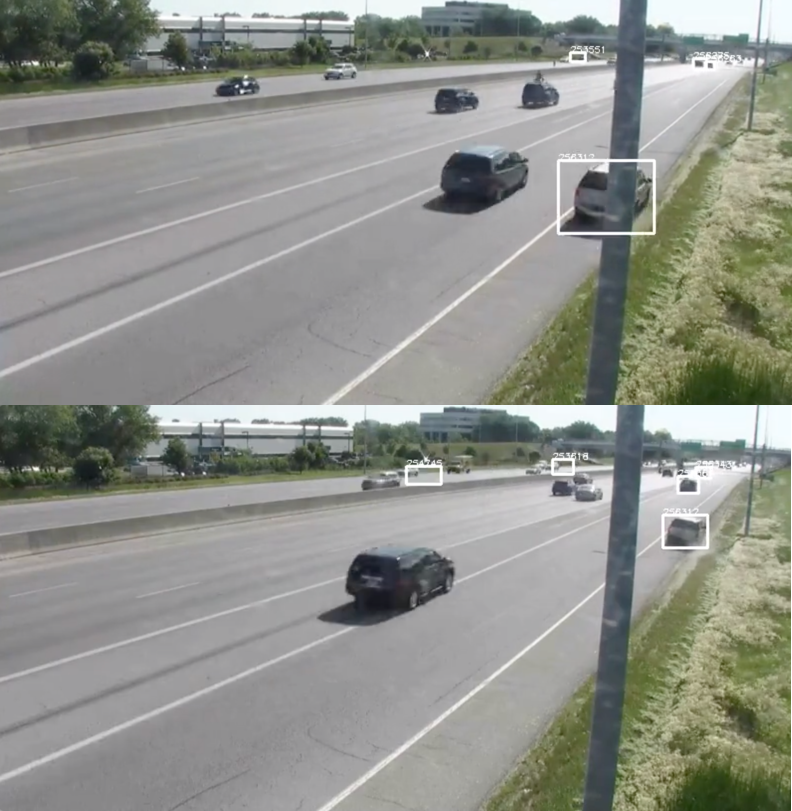
\includegraphics[width=8cm]{images/tracking_example1.png}
    \caption{A tracking result between 1st frame and 5th frame}
    \label{tracking_example2}
\end{figure}

Based on example \ref{tracking_example1}, we can observe id=256312 are moving in these five frames we found a relationship for this car among a sequential frames. We can exploit the moving information to verify if the car stalls or not and whether it's included in the road area or not. This car is an anomaly since it'll stay here in the remaining part. Moreover, we have more complicated situations like figure \ref{tracking_example2}, where there is a white care in the grass near the middle of the frame, so we cannot depend on our eyes. That's why our next section is about anomaly decision.

\begin{figure}  
    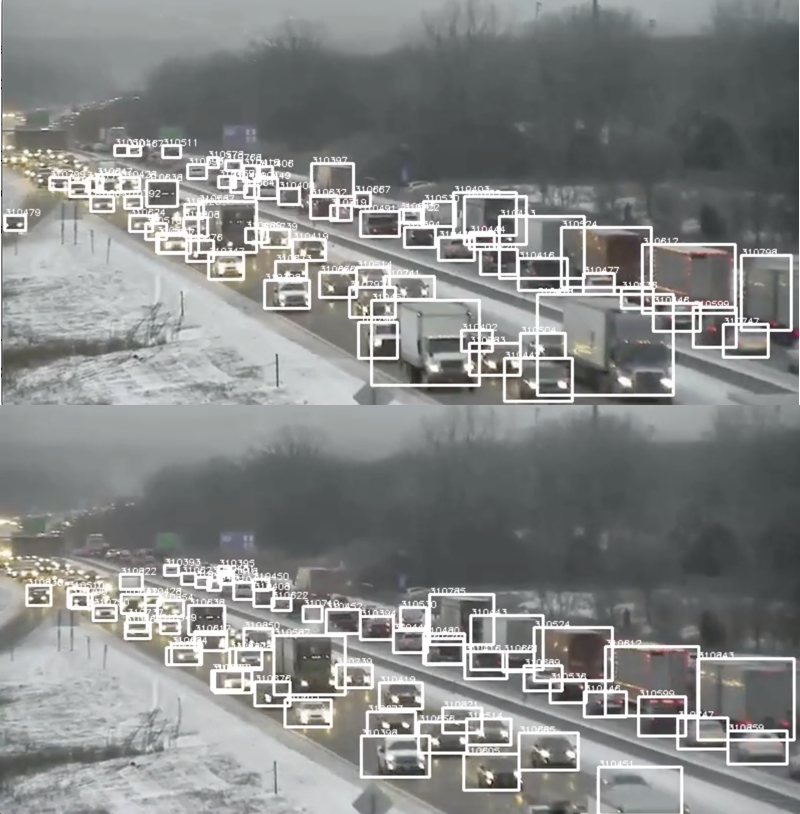
\includegraphics[width=8cm]{images/tracking_example2.png}
    \caption{Another more dense tracking result}
    \label{tracking_example1}
\end{figure}

\subsection{Anomaly detection based on histogram of pixels}
This way of approach is unsupervised learning. The key ideas are to divide the frame video into small regions having the size of $32 \times 32$. We calculate the change in pixel intensity in each small region to create the histogram of temporal features. This method is based on the assumption that if one anomaly happens, the histogram inside that region will be different from the rest of time frames. Although this approach is not generalize enough to cover all situations, it has decent results in most of cases.

\subsection{Anomaly calculation}
In this section, we demonstrate the anomaly calculation using cars and road relative position as well as the speed of each car. Since the tracking and detection results are not always correct, we leverage each car’s id to calculate their speed fluctuations and stopping duration in order to judge whether this is an anomaly event or not. We generate happening time as the output and compare it with the ground truth to measure our algorithm’s accuracy. Algorithm \ref{Anomal_Algo} shows the overall anomaly calculation in our approach.

\begin{algorithm}[!tbp]
\caption{Anomaly detection using relative position and speed}\label{Anomal_Algo}

\begin{algorithmic}[0]
\State \textbf{Input: Bounding boxes of cars, road and tracking} 
\State \textbf{Output: Anomaly time frame in the video} 
\end{algorithmic}

\begin{algorithmic}[1]

\State Convert the data into center position and speed form; [id, time, center, speed];
\State Subtract adjacent speed and position, and get the difference of positions and speed: DOP and DOS;
\State Set threshold for DOP and DOS and for ones lower that DOP and DOS, we set up them as 0;
\State Discard stationary objects(that could be a wrong detection) and discard unstable tracking, which means some trackings occur for a short time.
\State Discard the running cars during all the time and the stopping cars due to the traffic lights through a stopping time ratio threshold;
\State Merge anomalies at the same or close position. We think these cars crash due to the same reason;
\State Output the final anomalies .

\end{algorithmic}
\end{algorithm}


\section{Experimental results}
\subsection{Speed Validation}

After vehicle tracking, we have a sequence of each car that we've tracked in the last section. We assume the sequence is true (since we still face some tracking errors but we'll address it with a direction limitation in the next work). Since the camera position and perspective won't change, we can use the motion of the target centroid and the gap between frames in the videos to calculate the speed.

$$P(x, y) = \frac{(Box_{11} +  Box_{12} + Box_{11} +  Box_{22})}{4}$$

$$D(t) = \Sigma_{i=0}^{k}\frac{P_{t-i}}{k+1}$$

$$V(t) = \frac{D(t)}{gap}$$

\[
    h(x)= 
\begin{cases}
    1,& \text{if } V(t) > threshold\\
    0,              & \text{otherwise}
\end{cases}
\]
$P(x,y)$ is the representation of a target centroid, $D(t)$ is the average moving distance, and $V(t)$ represents the speed of a pixel's motion with the gap depending on the extracting rate from videos. The $h(x)$ classifies the anomalies and threshold based on the training results. So from this equation $h(x)$, we can know if a car stalls or not in the time $t$


\subsection{Road Detection}

Our cameras are all fixed meaning that the road will be static, and part of the background. This lets us use simple algorithms like Canny Edge Detection and Hough Transform to estimate the road areas in the each video. That's our subsequent work to finish.

After that, we'll compare whether the centroid of a car is in the area or not and then validate whether it ran off the road or not, which is the other type of anomaly we foresee needing to deal with. 

$$P(x, y) = \frac{(Box_{11} +  Box_{12} + Box_{11} +  Box_{22})}{4}$$
\[
    f(x)= 
\begin{cases}
    1,& \text{if } x\in Region_{road}\\
    0,              & \text{otherwise}
\end{cases}
\]

In this equation, P(x,y) represents the coordinates of the centroid of each car and $Region_{road}$ can be depicted with 0-1 Matrix. So the equation $f(P(x, y))$ will express whether it's an anomaly or not.

\subsection{Results and analysis}
\subsubsection{Qualitative}
The final goal of the model is to output the anomaly frame, all objects (cars) in each video frame need to be detected and tracked correctly. Figure \ref{detect_car} and \ref{detect_road} show some examples of our cars and road detection results. 

\begin{figure}  
    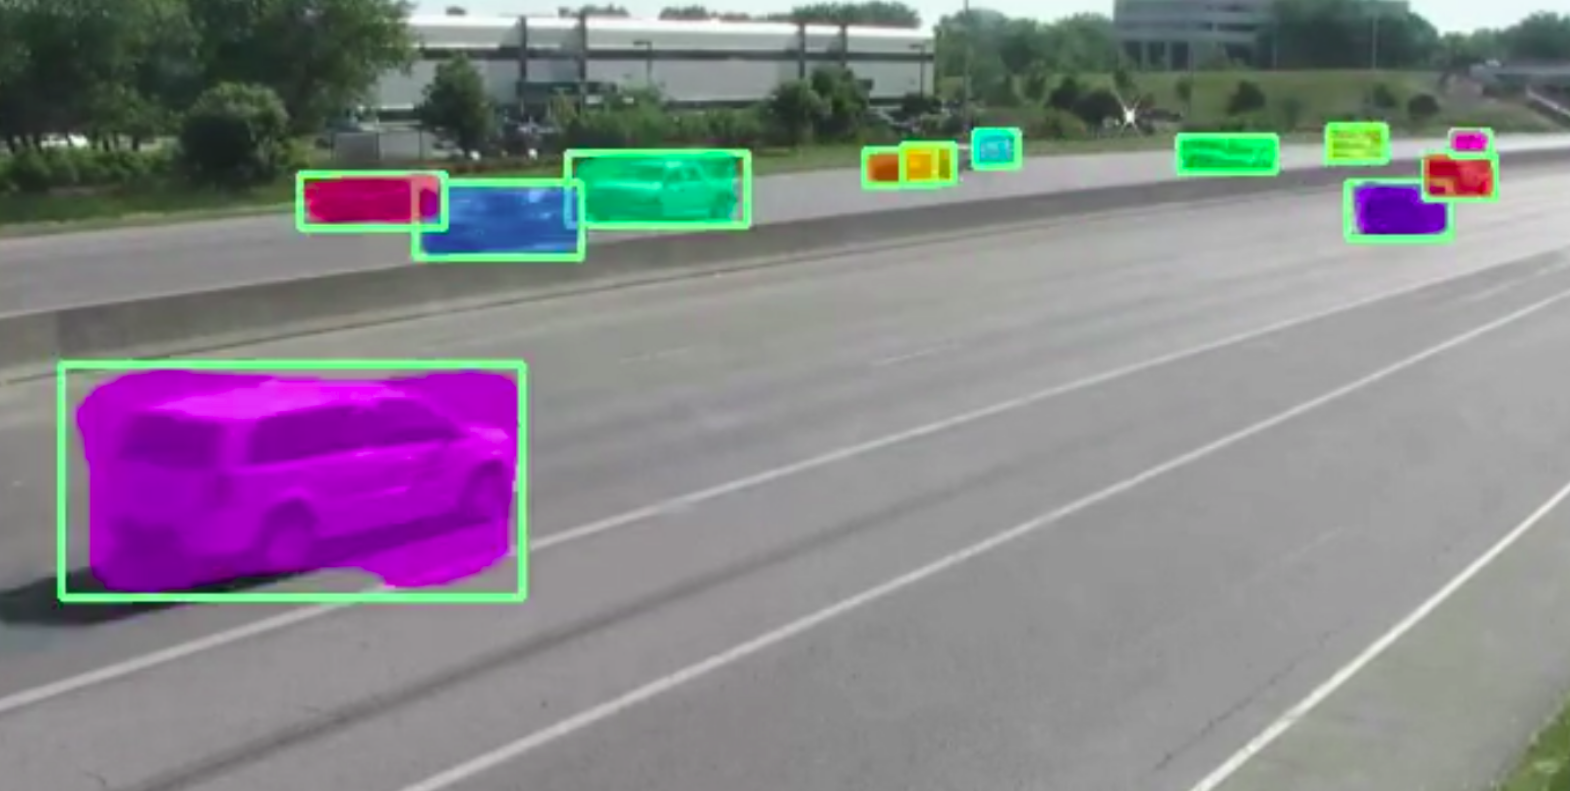
\includegraphics[width=8cm]{images/tunning1.png}
    \caption{Cars detection based on fine-tuning Mask-RCNN.}
    \label{detect_car}
	\end{figure}

\begin{figure}  
    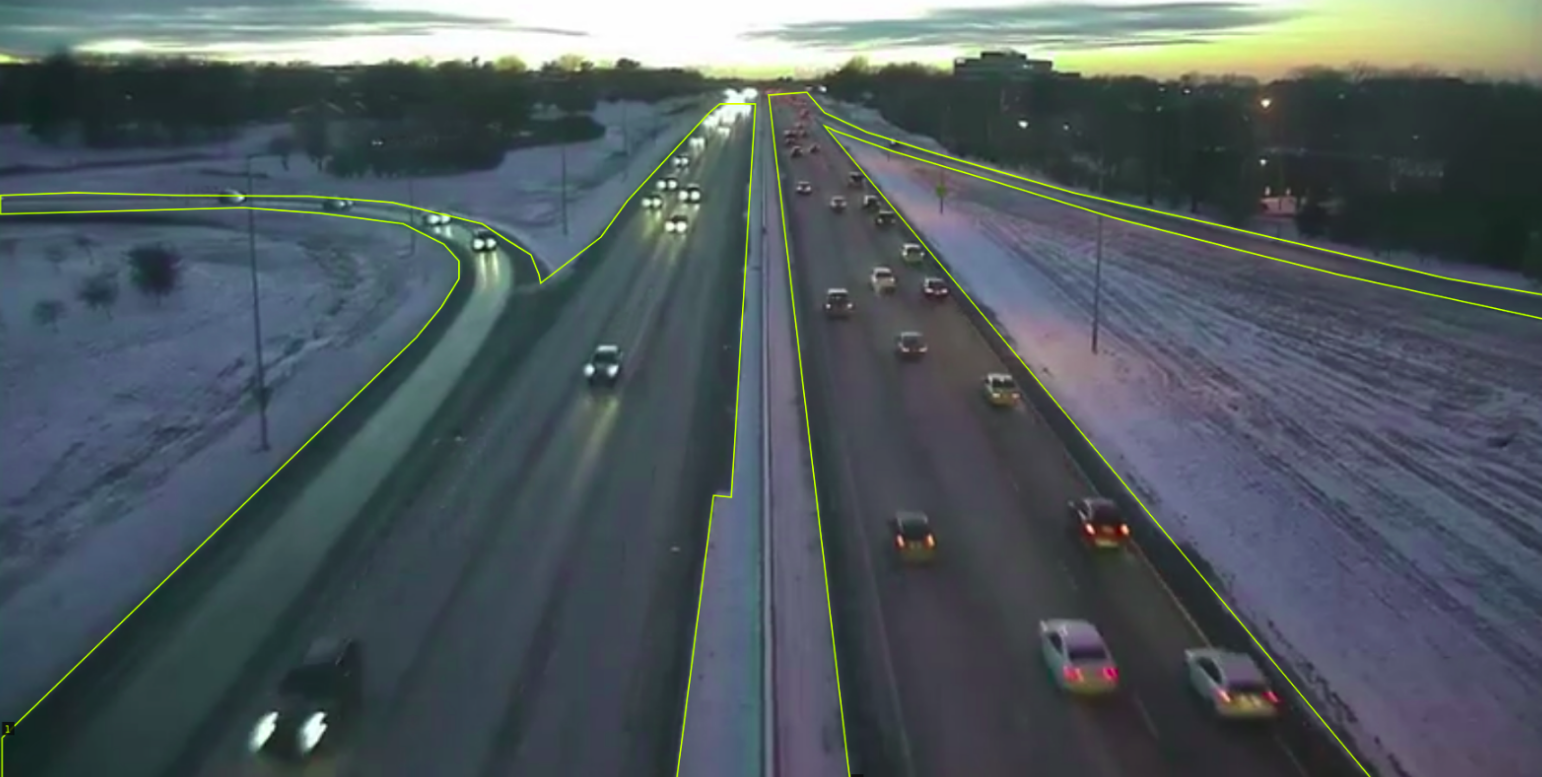
\includegraphics[width=8cm]{images/tunning2.png}
    \caption{Road detection based on relative fusion of cars position in frames.}
    \label{detect_road}
	\end{figure}

The difficulties in the data come from a whole host of problems. These include camera zooming and shakiness, illumination, differing camera viewpoints, poor quality videos, service roads with parking lots, and traffic lights. Figure \ref{diff_sis} shows some of these difficult situations.

\begin{figure}  
    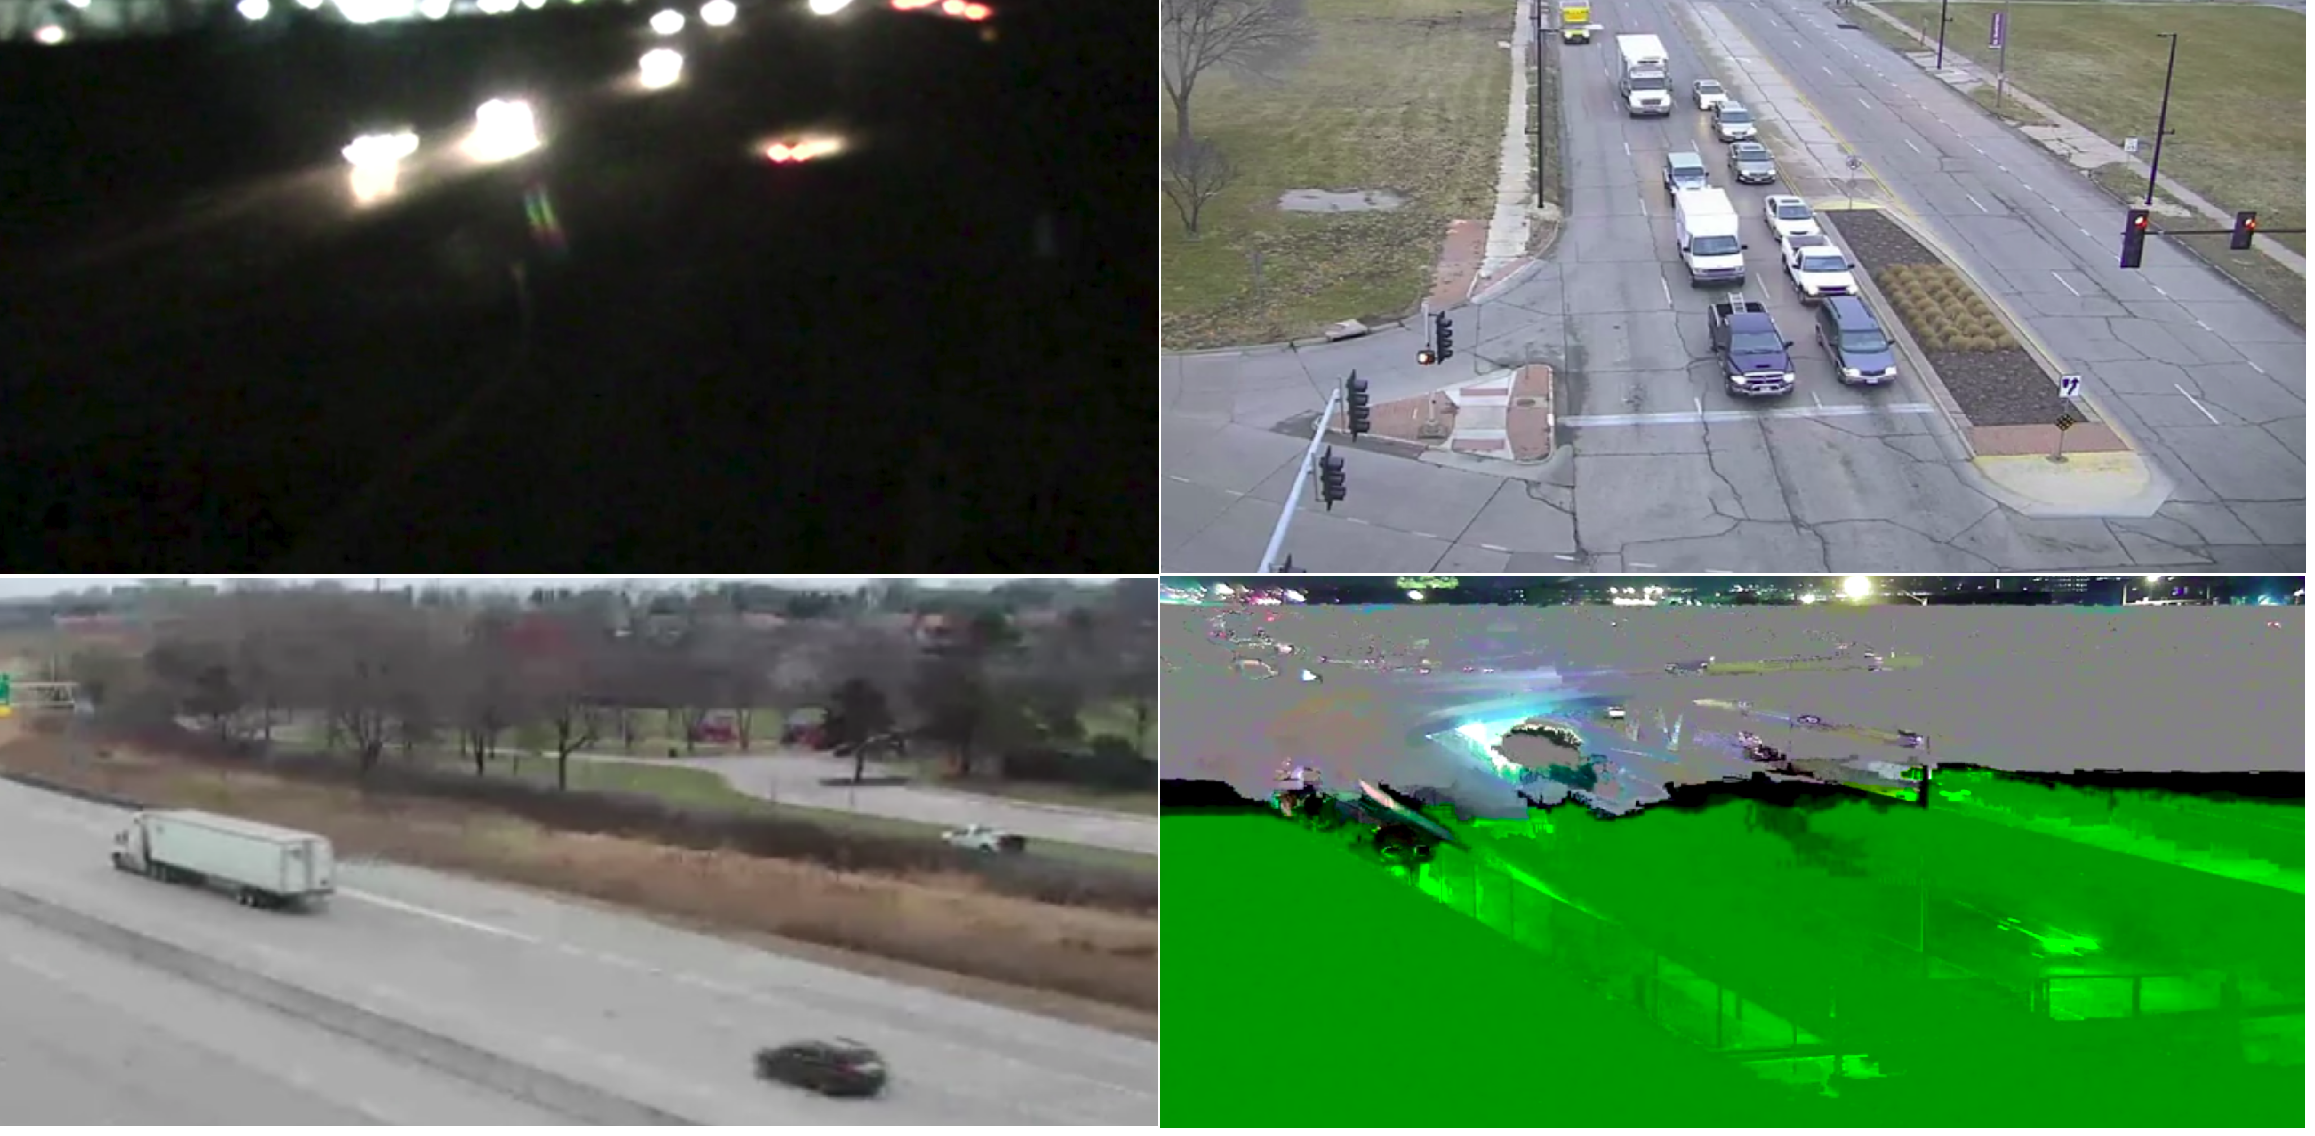
\includegraphics[width=8cm]{images/dif1.png}
    \caption{Some difficult situations in recored videos: different illuminations, viewpoints, errors between video frames, etc.}
    \label{diff_sis}
	\end{figure}

\subsubsection{Quantitative}
We used an F1-score to evaluate the correctness of the model for anomaly detection performance and detection time error, measured by RMSE. Specifically, the final score will be computed as $S_{Final}=F1 \times (1-NRMSE)$, where $F1$ is the F1-score and $NRMSE$ is the normalized root mean square error (RMSE). The score ranges between 0 and 1, and the higher scores reveal the better model.

For the purpose of computing the F1-score, a true-positive (TP) detection will be considered as the predicted anomaly within 10 seconds of the true anomaly (i.e., seconds before or after) that has the highest confidence score. Each predicted anomaly will only be a TP for one true anomaly. A false-positive (FP) is a predicted anomaly that is not a TP for some anomaly. Finally, a false-negative (FN) is a true anomaly that was not predicted.

We compute the detection time error as the RMSE of the ground truth anomaly time and predicted anomaly time for all TP predictions. Normalization will be done using min-max normalization with a minimum value of 0 and a maximum value of 300, which represents a reasonable range of RMSE values for the task. 

Figure \ref{res_quan} shows the quantitative results interactively of our model on validation set. 	
\begin{figure}  
    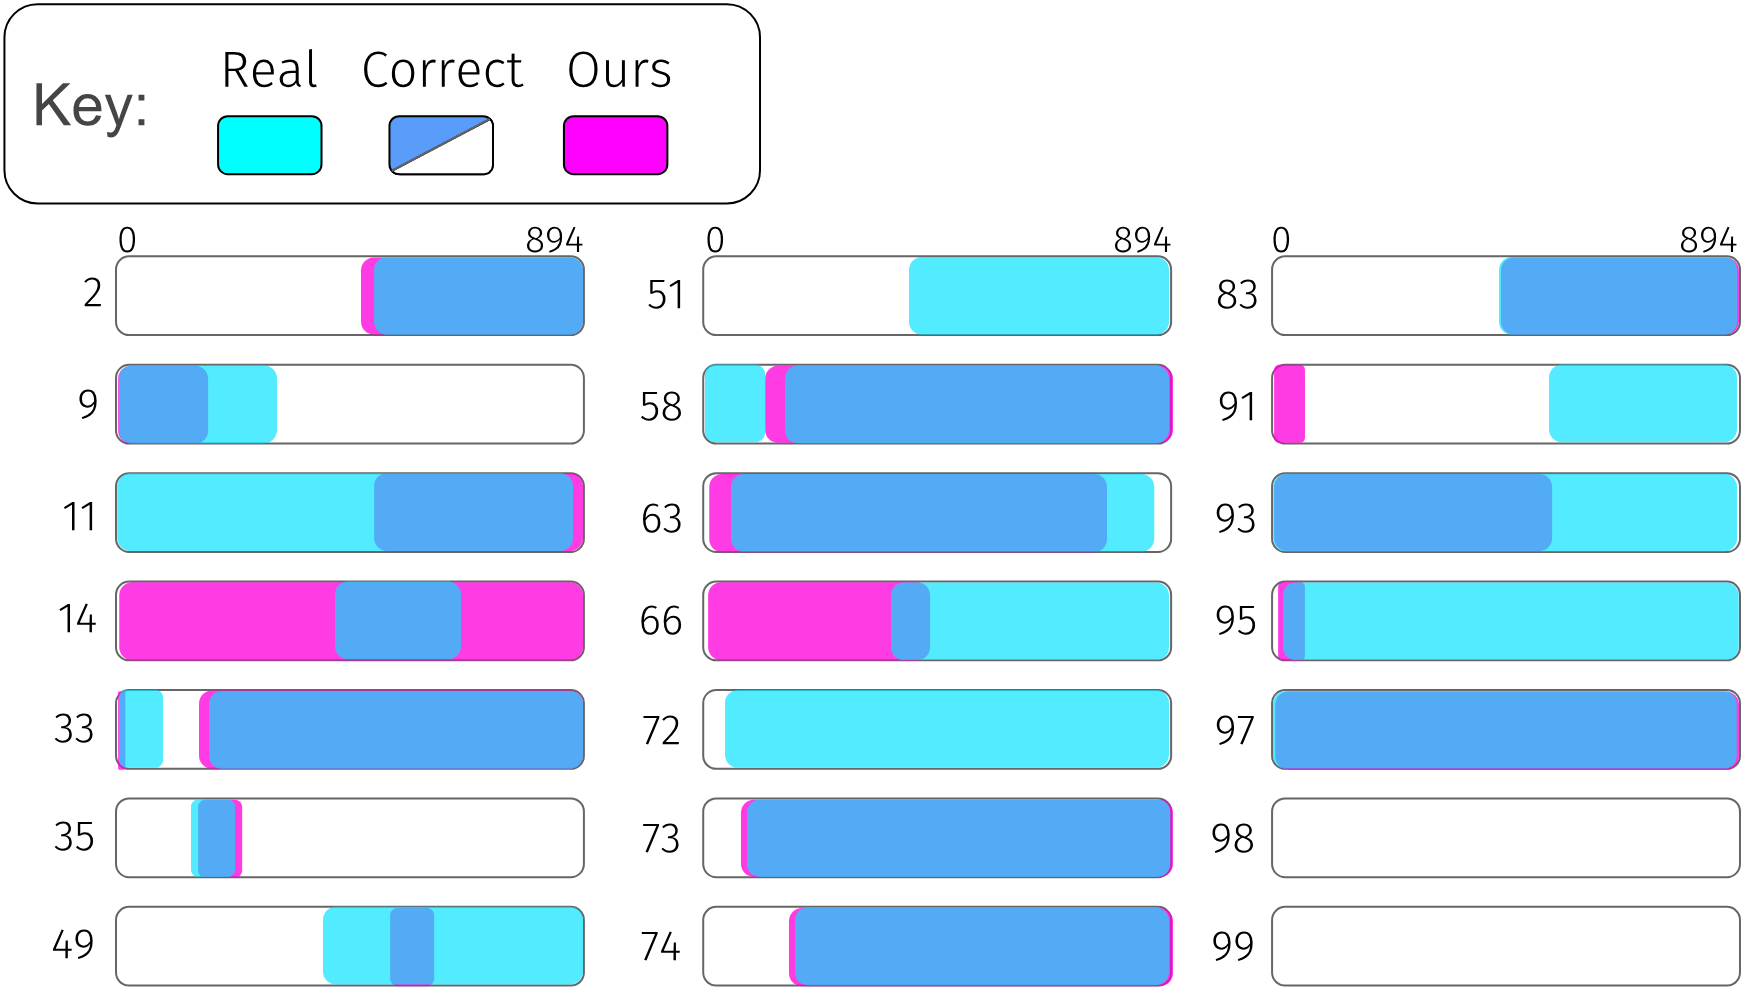
\includegraphics[width=8cm]{images/compare.png}
    \caption{Interactive quantitative comparison between our proposed model and validation set.}
    \label{res_quan}
	\end{figure}
	
\subsubsection{Profound Analysis}

During the experiment, we found tracking or detection result are not always good. Because we cannot detect each vehicle in the video and the algorithm also will detect some wrong objects as vehicles, which can cause some false positive cases. For our tracking module, the identity of objects will change if there is an overlap with trucks or other big cars. Our algorithm will label one object with two or more identities. These two cases can cause faults directly. However, there are some fixed patterns in our traffic flow videos. For example, the stalling can keep stationary for a long time and at this time, the identity won't change due to overlap or lost focus. Thus, our tracking algorithm cannot achieve a very high accuracy but fortunately, we can leverage the features above to capture exact anomalies. We'll look into that reason more in the future.

\section{Conclusion and future Work}

We have presented the model and architecture for the anomaly detection. The proposed approach contains three modules: 1) We leverage Mask R-CNN, a state-of-the-art semantic segmentation network, to detect cars which are likely to be anomalies; 2) We extract each patch based on the output of last section and use cosine similarity to build a relationship between two continuous frames; 3) In terms of speed estimation and position comparison with other auxiliary like road detection, we can judge if the stalling vehicle crashed or it just stops due to the traffic light. Experimental results show that our approach can get correct results in almost all videos. It also has fairly small differences compared to the ground truth. We believe that our approach method can be used as a based line for anomaly detection development in the future. 

During the tracking part, we still have a large space to improve the accuracy because we only use cosine similarity to capture the correlation between patches. In the future, we can compare more methods like CNN to find the correspondence of vehicles and improve our performance. Furthermore, the parameters in the anomaly decision part can be learned through LDA if we can get more videos and not just depend on our obversation and some empirical data.


{\small
\bibliographystyle{ieee}
\bibliography{egbib}
}

\end{document}
